\documentclass[a4paper,oneside,DIV=12,12pt,headings=normal]{scrartcl}

%%% Length calculations
\usepackage{calc}
%%%

%%% Support for color
\usepackage{xcolor}
\definecolor{lightblue}{HTML}{03A9F4}
\definecolor{red}{HTML}{F44336}
%%%

%%% Graphics inclusion
\usepackage{graphicx}
%%%

%%% Font selection
\usepackage{fontspec}

\setromanfont{STIX Two Text}[
	SmallCapsFeatures = {LetterSpace = 5},
]

\setsansfont{Source Sans Pro}[
]

\setmonofont{Source Code Pro}[
]
%%%

%%% Math settings
\usepackage{amsmath,unicode-math}
\setmathfont{STIX Two Math}

% \usepackage{IEEEtrantools}
\usepackage{mleftright}
%%%

%%% Font settings for different KOMA Script elements
\setkomafont{pagenumber}{\rmfamily}
\setkomafont{disposition}{\rmfamily\bfseries}
%%%

%%% Typographic enhancements
\usepackage{microtype}
%%%

%%% Language-specific settings
\usepackage{polyglossia}
\setmainlanguage{ukrainian}
%%%

%%% List settings
\usepackage{enumitem}
\setlist[enumerate]{
	leftmargin = *,
}
%%%

%%% Captions
\usepackage{caption}
\usepackage{subcaption}

\DeclareCaptionLabelFormat{closing}{#2)}
\captionsetup[subtable]{labelformat = closing}
\captionsetup[subfigure]{labelformat = closing, position = auto}
%%%

%%% Tables
\usepackage{booktabs}
\usepackage{longtable}

\usepackage{multirow}

\usepackage{array}
\newcolumntype{v}[1]{>{\raggedright\arraybackslash\hspace{0pt}}p{#1}}
\newcolumntype{b}[1]{>{\centering\arraybackslash\hspace{0pt}}p{#1}}
\newcolumntype{n}[1]{>{\raggedleft\arraybackslash\hspace{0pt}}p{#1}}

\usepackage{kbordermatrix} % labeling array indices
%%%

%%% Floats on a single row
\usepackage{floatrow}
\newfloatcommand{capbtabbox}{table}[][\FBwidth]
%%%

%%% Links and hyperreferences
\usepackage{hyperref}
\hypersetup{
	colorlinks      = false,
	linkbordercolor = red,
	urlbordercolor  = lightblue,
	pdfborderstyle  = {/S/U/W 1.5},
}
%%%

%%% All caps
\newcommand{\allcaps}[1]{{\addfontfeatures{LetterSpace = 3}#1}}
%%%

%%% Ceiling function typesetting
\newcommand{\ceil}[1]{\mleft\lceil#1\mright\rceil}
%%%

\begin{document}
	\begin{titlepage}
	\centering
		Міністерство освіти і науки України\\
		Національний авіаційний університет\\
		Навчально-науковий інститут комп'ютерних інформаційних технологій\\
		Кафедра комп'ютеризованих систем управління

		\vspace*{\fill}

		Лабораторна робота №4\\
		з дисципліни «Архітектура комп'ютерів»\\
		на тему «Проектування запам'ятовуючих пристроїв»\\
		Варіант №4

		\vspace*{\fill}
		
		\begin{flushright}
			Виконав:\\
			студент ННІКІТ СП-225\\
			Клокун В.\,Д.\\
			Перевірив:\\
			Зіньков Ю.\,Г.
		\end{flushright}

		Київ 2018
    \end{titlepage}

		\section{Мета роботи}
			Оволодіти знаннями та практичними навичками з проектування запам'ятовуючих пристроїв на базі \allcaps{ПЛІС} типу \allcaps{FPGA}.

		\section{Хід роботи}
			Створюємо запам'ятовуючий пристрій, який розрахований на підтримку таких параметрів:
			\begin{enumerate}
				\item FIFO.
				\item Єдине тактування для зчитування та запису.
				\item Додаткові сигнали заповнення, пустоти, лічильника зайнятих комірок.
				\item Розрядність~— 32.
				\item Число комірок~— 32.
			\end{enumerate}
			Спроектуємо схему необхідного запам'ятовуючого пристрою.
			\begin{figure}[!htbp]
				\centering
				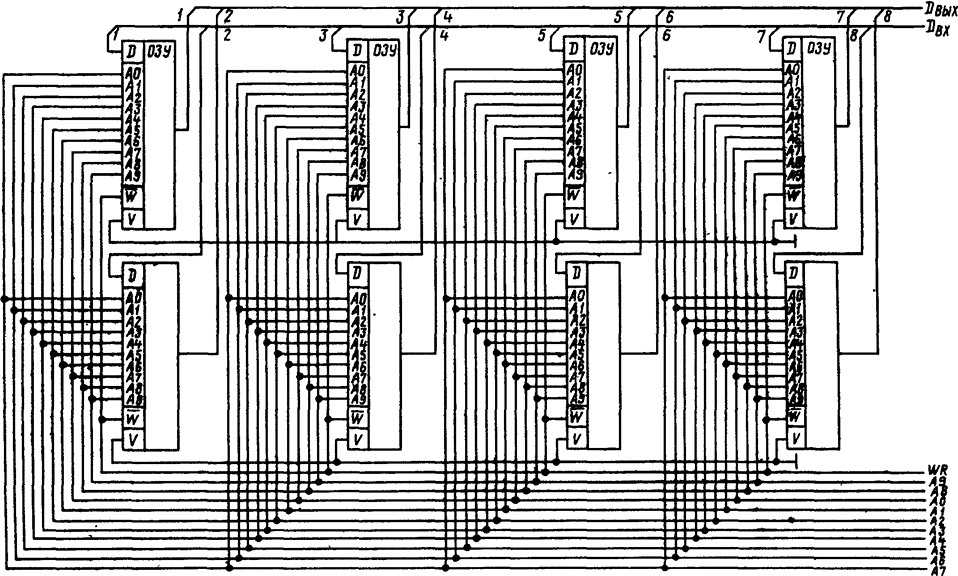
\includegraphics[width = \linewidth]{./assets/01.png}
				\caption{Схема, під яку спроектовано пристрій}
				\label{fig:schematic-01}
			\end{figure}
			
			Для розуміння кожного з елементів, зображених на схемі~(рис.~\ref{fig:schematic-01}) необхідно представити елемент у відповідному вигляді~(рис.~\ref{fig:schematic-02}). Бачимо, що такий підхід до реалізації вимагає відповідну схему (рис.~\ref{fig:schematic-03}).

			\begin{figure}[!htbp]
				\centering
				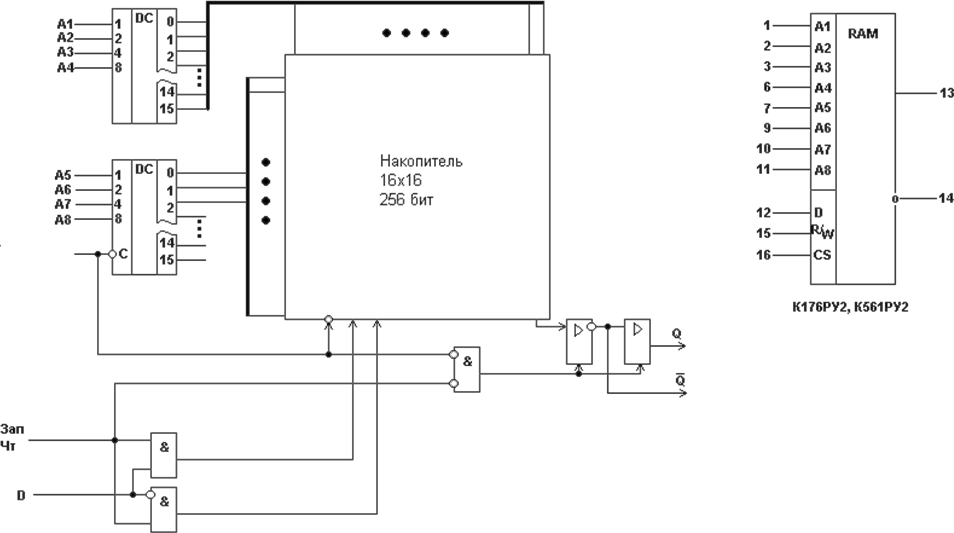
\includegraphics[width = \linewidth]{./assets/02.png}
				\caption{Схема для покращеного розуміння}
				\label{fig:schematic-02}
			\end{figure}

			\begin{figure}[!htbp]
				\centering
				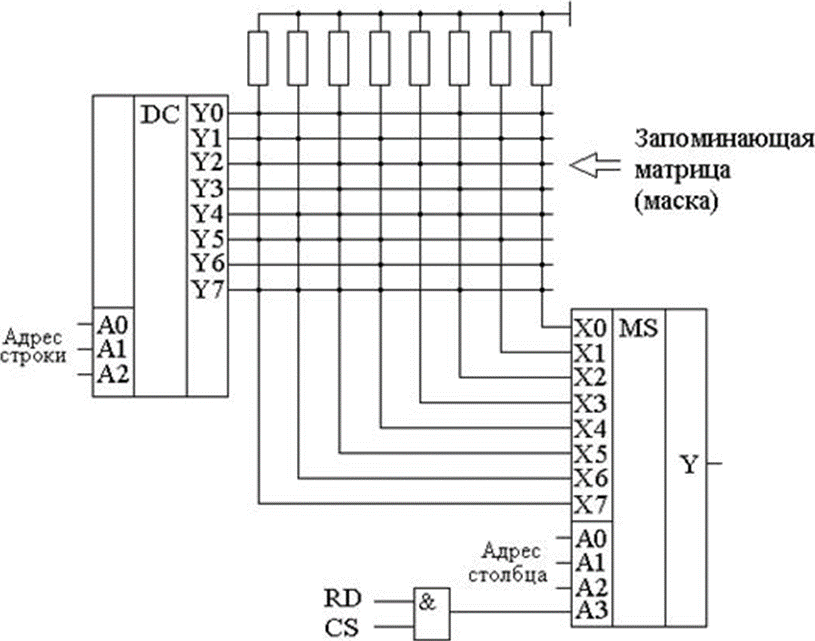
\includegraphics[height = 17\baselineskip]{./assets/03.png}
				\caption{Реалізація запам'ятовуючого пристрою}
				\label{fig:schematic-03}
			\end{figure}

			Після проектування пристрою необхідно перевірити правильність його роботи. Виконаємо перевірку табличним методом~(табл.~\ref{tab:test-table}).

			\begin{table}[!htbp]
				\centering
				\begin{tabular}{r|*{9}{c}}
					\toprule
					  & 1 &  2 &  3 &  4 &  5 &  6 &  7 &  8 &  9 \\
					\midrule
					1 & 1 &  2 &  3 &  4 &  5 &  6 &  7 &  8 &  9 \\
					2 & 2 &  4 &  6 &  8 & 10 & 12 & 14 & 16 & 18 \\
					3 & 3 &  6 &  9 & 12 & 15 & 18 & 21 & 24 & 27 \\
					4 & 4 &  8 & 12 & 16 & 20 & 24 & 28 & 32 & 36 \\
					5 & 5 & 10 & 15 & 18 & 25 & 30 & 35 & 40 & 45 \\
					6 & 6 & 12 & 18 & 24 & 30 & 36 & 42 & 48 & 54 \\
					7 & 7 & 14 & 21 & 28 & 35 & 42 & 49 & 56 & 63 \\
					8 & 8 & 16 & 24 & 32 & 40 & 48 & 56 & 64 & 72 \\
					9 & 9 & 18 & 27 & 36 & 45 & 54 & 63 & 72 & 81 \\
					\bottomrule
				\end{tabular}
				\caption{Таблиця перевірки роботи пристрою}
				\label{tab:test-table}
			\end{table}

			\section{Висновок}
				Під час виконання даної лабораторної роботи ми отримали знання та~оволоділи практичними навичками проектування запам'ятовуючих пристроїв на~базі \allcaps{ПЛІС} типу~\allcaps{FPGA}.

\end{document}

